\chapter{Receiver Design}
\section{Receiver Architecture}
\subsection{Quadrature Baseband Sampling Receiver}
The most simple and
\begin{itemize}
\item Show overview picture of architecture
\item Frequency space pictures of Baseband, TX-IF, 60G, RX-IF, Baseband
\item Con: LO Self-Mixing leads to DC-Offset that has to be blocked using a
  High-Pass-Filter also removes a small part of the signal
\end{itemize}

\begin{figure}[ht]
  \centering
  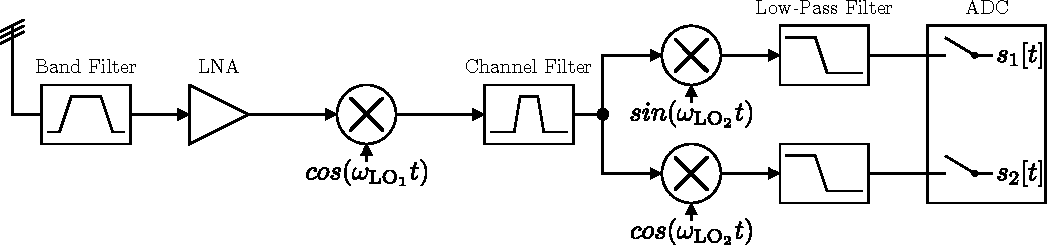
\includegraphics[width=\textwidth]{figures/quad_base_rx_block_diagram}
  \caption{Block Diagram of Quadrature Baseband Sampling Receiver}
  \label{fig:rx_quad_base_bd}
\end{figure}

\subsection{Intermediate Frequency Sampling Receiver}
\begin{itemize}
\item Show overview picture of architecture
\item Frequency space pictures of Baseband, TX-IF, 60G, RX-IF, Baseband
\item RX and TX-LO offset to make sure LSB part is out of band
\end{itemize}

\begin{figure}[ht]
  \centering
  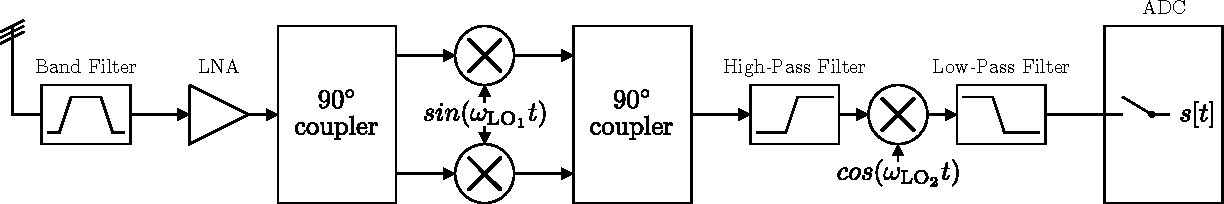
\includegraphics[width=\textwidth]{figures/if_rx_block_diagram}
  \caption{Block Diagram of Intermediate Frequency Sampling Receiver}
  \label{fig:rx_if_bd}
\end{figure}

\subsection{Quadrate Intermediate Frequency Sub-Nyquist Sampling Receiver}
\begin{itemize}
\item Show overview picture of architecture
\item Motivation: Save external mixer
\item Frequency space pictures of Baseband, TX-IF, 60G, RX-IF, Baseband
\item Sub-nyquist sampling, reference to component restrictions
\item Show how sub-nyquist sampling works with hilbert transform to generate analytical signal
\end{itemize}

\begin{figure}[ht]
  \centering
  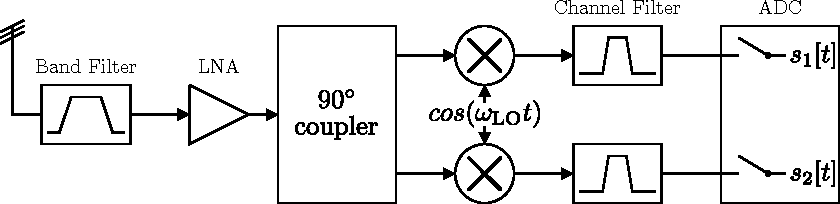
\includegraphics[width=\textwidth]{figures/quad_if_rx_block_diagram}
  \caption{Block Diagram of Quadrate Intermediate Frequency Sub-Nyquist Sampling Receiver}
  \label{fig:rx_quad_if_bd}
\end{figure}

\section{Generation of Analytic Signal In Analog Domain}
\begin{itemize}
\item Explain how perfect analytic signal is created using hilbert transform
\item Explain how it is created using the sin/cos mixer
\item Explain error introduced in non perfect case
\end{itemize}
